%!TEX root = ../slides.tex
\section{Implementation}
%\subsection{Implementation}
\begin{frame}{Implementation}{Android device implementation}
\small

\begin{block}{\small \textbf{Smartphone device}}
The Google Nexus 6 smartphone with Android 7 was employed.
\begin{itemize}
  \item Quad-core 2.7 GHz Krait 450 mobile processor (Qualcomm Snapdragon 805 chipset).
  \item 3 GB RAM.
  \item Qualcomm Snapdragon 805 chipset.
  \item 3220 mAh battery.
\end{itemize}
\end{block}

\begin{alertblock}{\small \textbf{Technical barriers}}
\begin{enumerate}
  \item Asynchronous access to sensors, affected by sensing infrastructure (GPS satellite signal intermittency).
  \item Out-of-the-box energy saving mechanisms:
  \begin{itemize}
    \item Application specific: \textbf{App StandBy}.
    \item System wide: \textbf{Doze mode}.
  \end{itemize}
\end{enumerate}
\end{alertblock}

\begin{exampleblock}{\small \textbf{Workarounds}}
\begin{enumerate}
  \item Grace periods for sampling (\texttt{Timer} + \texttt{TimerTasks}).
  \item \texttt{Alarms}, \texttt{WakeLocks}, foreground services.
\end{enumerate}
\end{exampleblock}
\end{frame}

{\aauwavesbg%
  \begin{textblock*}{5cm}(0.3cm,0.3cm)
  \small
  \textbf{The architecture of the proposed system implemented in the Android software stack.}
  \end{textblock*}
\begin{textblock*}{1cm}(12cm,9.3cm)
  \scriptsize
  \insertframenumber~/~\inserttotalframenumber
  \end{textblock*}
\begin{frame}[plain]
  \centering
  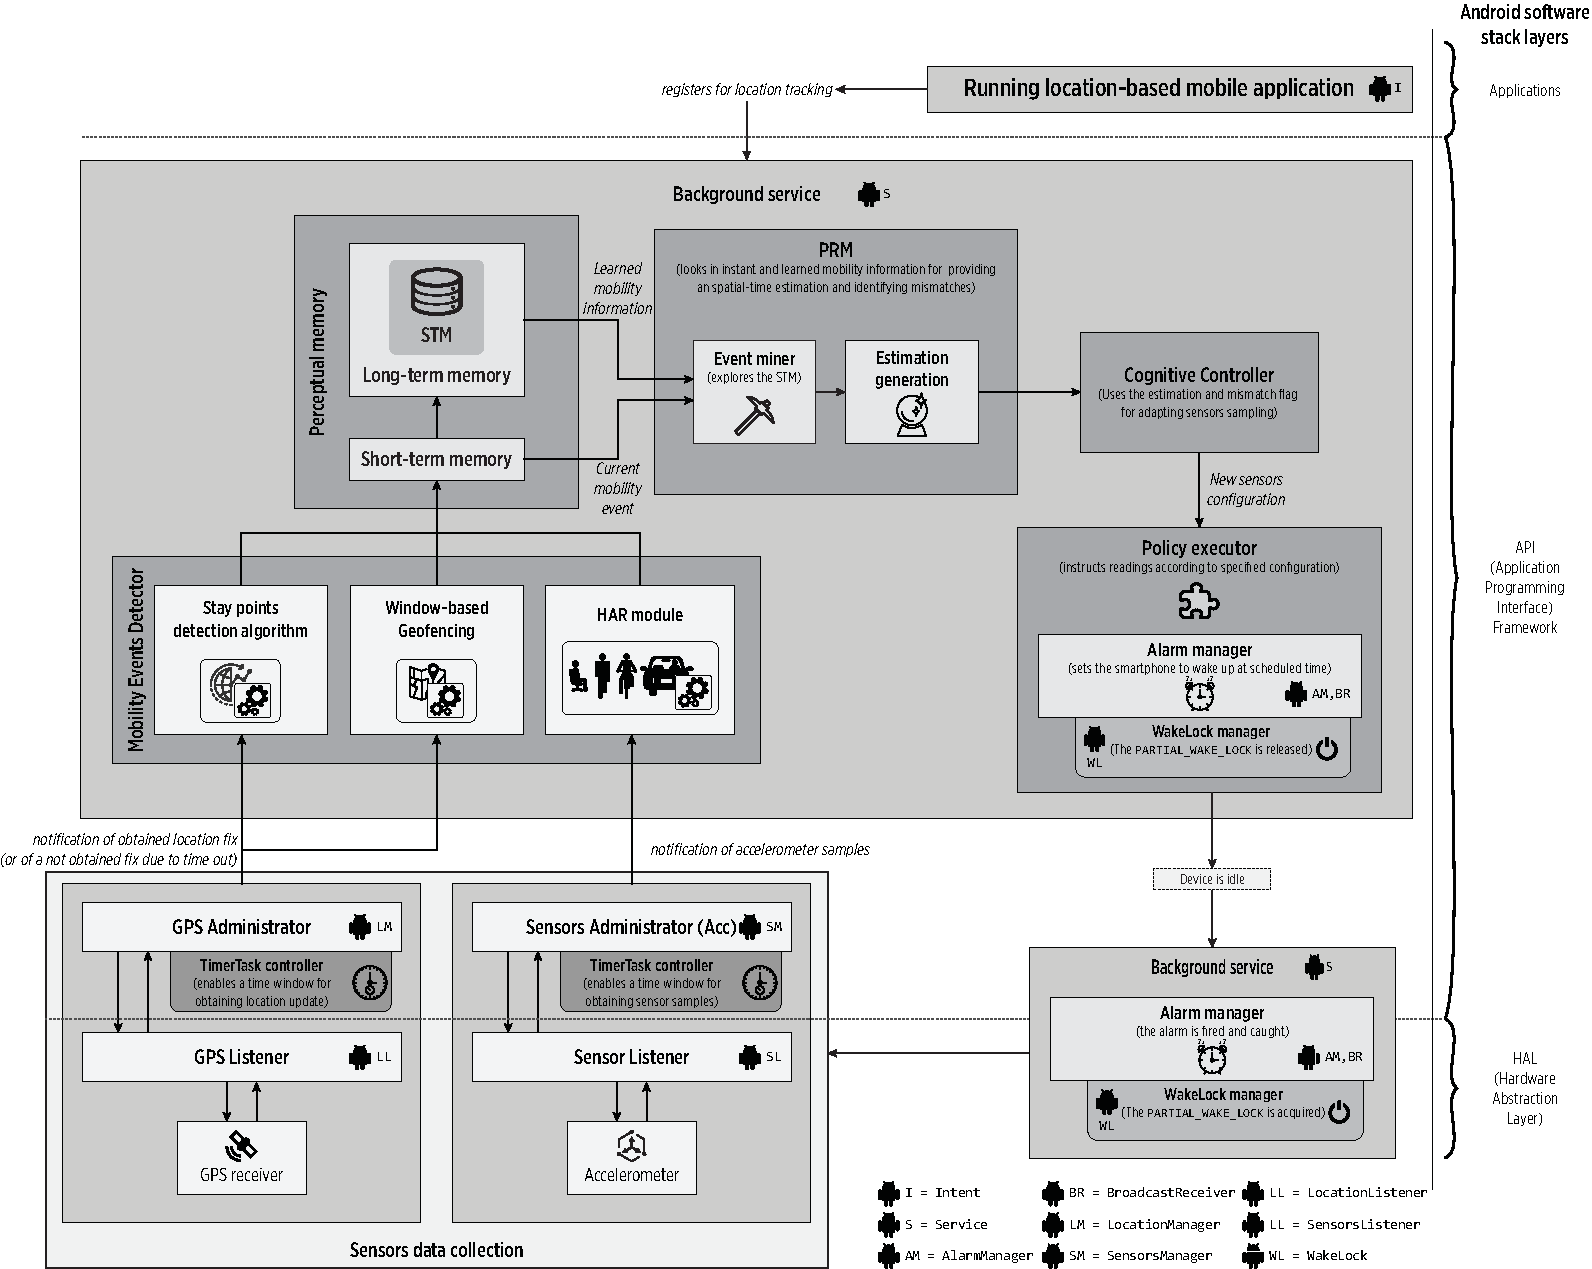
\includegraphics[width=\textwidth]{vectors/implementation}
\end{frame}}

% \begin{frame}{Implementation}{Android device implementation}
% \begin{center}
% 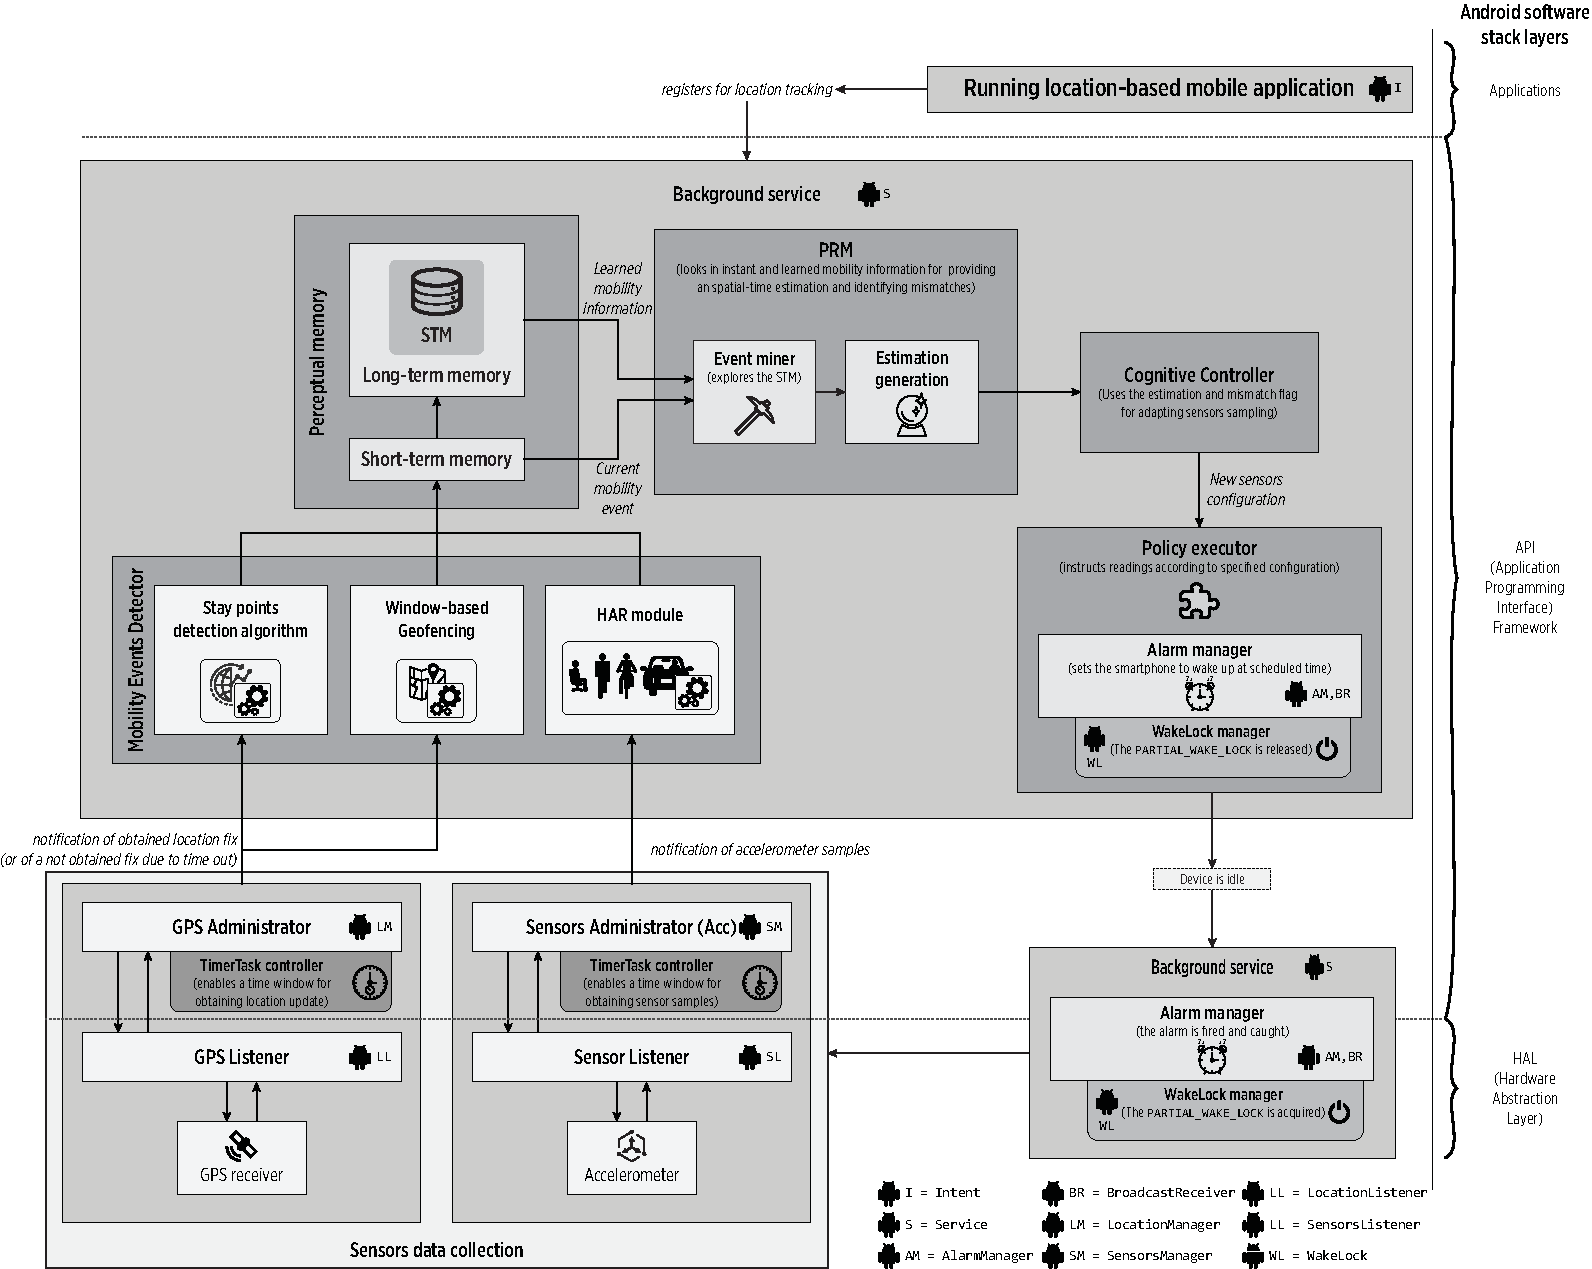
\includegraphics[width=0.8\textwidth]{vectors/implementation}
% \end{center}
% \end{frame}